%-------------------------------------------------------------------------------
% Document setup, template definition
%-------------------------------------------------------------------------------

% Language, encoding and paper size
\documentclass[a4paper]{article}
\usepackage{polyglossia}
\setmainlanguage{slovak}
\usepackage{fontenc}

% Packages
\usepackage{fancyhdr}
\usepackage{extramarks}
\usepackage{lastpage}
\usepackage{amsmath,amsthm}
\usepackage{amsfonts}
\usepackage{mathtools}
\usepackage{pgf}
\usepackage{tikz}
\usepackage{bm}
\usepackage{mathrsfs}

\usepackage{marginnote}

% Margins, page size, ...
\voffset=-1in
\topmargin=0.5cm
\textheight=27cm
\headsep=0.5cm
\hoffset=-1in
\evensidemargin=1.5cm
\oddsidemargin=1.5cm
\textwidth=18cm

% Header and footer
\pagestyle{plain}
%\lhead{\tplName}
%\chead{\textsc{\tplClass}: \tplTitle}
%\rhead{\tplDate}
%\cfoot{}
%\rfoot{Strana \thepage\ z\ \pageref{LastPage}}

% Size of the header/footer rule
\renewcommand\headrulewidth{0.4pt} 
\renewcommand\footrulewidth{0.4pt}

%-------------------------------------------------------------------------------
% Custom definitions (shortcuts, ...)
%-------------------------------------------------------------------------------
\let\eps=\varepsilon % definujeme si pekne epsilon
\let\then=\Rightarrow % krok odvodenia
\def\kodTS#1{{\tt <}#1{\tt >}}
\newcommand{\bigO}[1]{\ensuremath{\mathcal{O}(#1)}}


%-------------------------------------------------------------------------------
% Template variables - Name, Class, Date, ...
%-------------------------------------------------------------------------------
%\newcommand{\tplName}{Ladislav Pápay}
%\newcommand{\tplGroup}{}
%\newcommand{\tplClass}{VZV}
%\newcommand{\tplTitle}{Domáca úloha 2.1}
%\newcommand{\tplDate}{19.10.2014}

%-------------------------------------------------------------------------------
% Document contents
%-------------------------------------------------------------------------------

%\newtheorem{zadanie}{Zadanie}[section]
\newenvironment{zadanie}{\trivlist\item[\hskip \labelsep{\bfseries Zadanie:}]}{\endtrivlist}
\newenvironment{konstrukcia}{\trivlist\item[\hskip \labelsep{\bfseries Konštrukcia:}]}{\endtrivlist}
\newenvironment{dokaz}{\trivlist\item[\hskip \labelsep{\bfseries Dôkaz:}]}{\endtrivlist}
\newenvironment{rozhodnutie}{\trivlist\item[\hskip \labelsep{\bfseries Rozhodnutie:}]}{\endtrivlist}
\newenvironment{priklad}{\trivlist\item[\hskip \labelsep{\bfseries Príklad:}]}{\endtrivlist}
\newtheorem{lema}{Lema}[section]

\usepackage{adjustbox}

\begin{document}
\begin{description}
\item[Hash functions] \hfill
	\begin{description}
		\item[MD5] 128bit digest, 64=4x16 rounds, 32bit, each round: s[]=shifts K[]=constants $ \lfloor |sin(i+1)\cdot2^{32}| \rfloor$. \hfill\\
			Input 512bit blocks, padding+64bit length\\
			$F_1 = (B\land C)\lor(\overline{B}\land B)$, $F_2 = (B\land D)\lor(C\land\overline{D})$, $F_3 = (B\oplus C \oplus D)$, $F_4 = C \oplus (B \lor\overline{D})$\\
			$2^{18}$ collisions, <1 sec
		\item[SHA1] 160bit, 80=4x20 rounds, 32bit, theoretical collisions $2^{60}$.
		\item[SHA2] 256/512bit=8*32/64, 512/1024 blocks, 64/80 rounds, reduced rounds preimage/collision \hfill\\
			Ch = choice, $(E \land F)\oplus(\overline{E} \land G)$, Ma = majority $(A \land B)\oplus(A \land C)\oplus(B \land C)$ \\
			$\Sigma$ = rotations + xor
	\end{description}
	\begin{minipage}[t]{\linewidth}
	\raggedright
		\adjustbox{valign=t}{%
			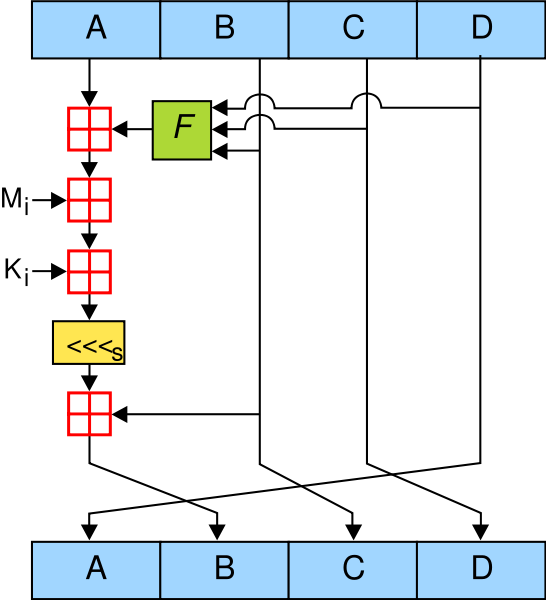
\includegraphics[height=0.3\linewidth]{md5.png}\hspace{0.5cm}%
			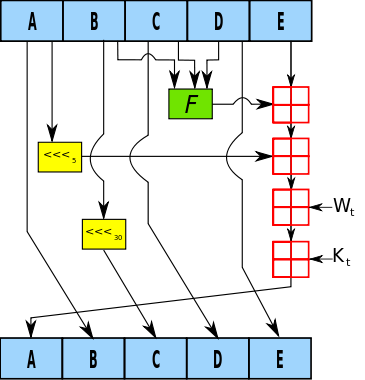
\includegraphics[height=0.3\linewidth]{sha1.png}\hspace{0.5cm}%
			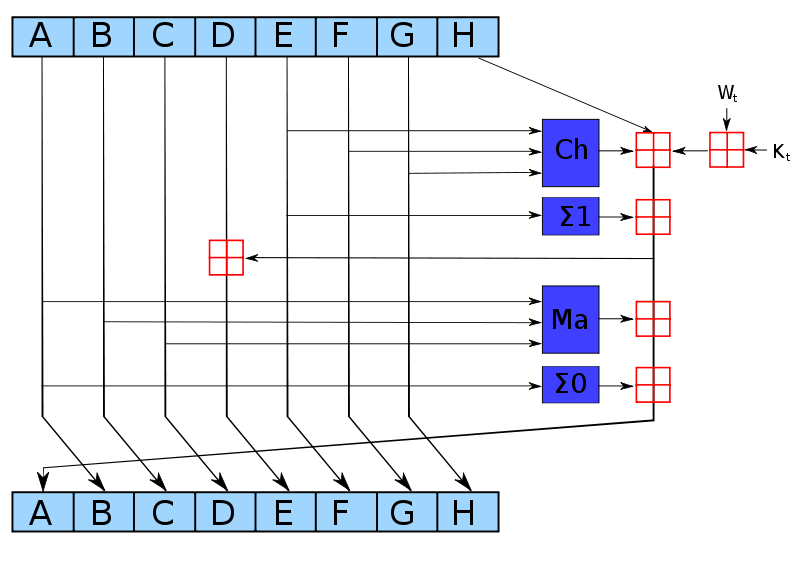
\includegraphics[height=0.3\linewidth]{sha2.png}%
		}
	\end{minipage}
\item[SAT solvers] \hfill
	\begin{description}
		\item[Naive]
		\item[DPLL] Davis-Putnam-Logemann-Loveland; Two rules at each step \hfill
			\begin{description}
				\item[Unit propagation] unit = clause with 1 unassigned literal \hfill\\
					If clause is satisfied, ignore. If not, use the only possible assignment for the unassigned literal.
				\item[Pure literal elimintaion] pure literal = single polarity in all clauses \hfill\\
					Can assign the required value and then ignore.
			\end{description}
		\item[CDCL] Conflict-Driven Clause Learning \hfill
			\begin{description}
				\item[Implication graph] directed, vertices are literals + assignment \hfil\\
					\textbf{Decision} (normal step) or \textbf{Forced} (one of DPLL two rules)
					When in conflict, find the responsible literals (forced), build new \textbf{Learnt clause}, add to rest. Backtrack to point when first of conflict variables was assigned. (nonchronological backtracking) \\
					\begin{minipage}[t]{\linewidth}
						\raggedright
						\vspace{-0.5cm}
						\adjustbox{valign=t}{%
							\hspace{11cm}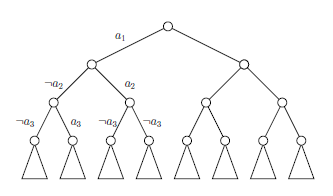
\includegraphics[width=0.25\linewidth]{cdcl1.png}%
						}
					\end{minipage}
					\begin{minipage}[t]{\linewidth}
						\raggedright
						\adjustbox{valign=t}{%
							\hspace{11cm}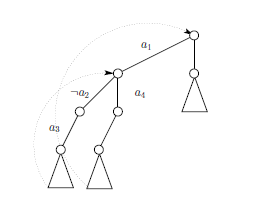
\includegraphics[width=0.25\linewidth]{cdcl2.png}%
						}
					\end{minipage}
					\vspace{-5cm}
			\end{description}
	\end{description}
\item[Encoding] \hfill
	\begin{description}
		\item[Existing] Vegard Nossum 2012 Uni of Oslo - SAT-based preimage SHA1 \hfill\\
			Code: 1000 lines C++, ~120 lines sha1, ~40 lines compression function
		\item[Boolean circuit] - recursively expand/substitute - exponential in circuit size
		\item[Tseitin transformation] - helper variables for each node in circuit
			\begin{description}
				\item[AND] $A\land B$ $(C \lor \overline{A} \lor \overline{B}) \land (\overline{C} \lor A) \land (\overline{C} \lor B)$
				\item[OR] $A\lor B$ $(\overline{C} \lor A \lor B) \land (C \lor \overline{A}) \land (C \lor \overline{B})$
				\item[XOR] $A\oplus B$ $(\overline{C} \lor \overline{A} \lor \overline{B}) \land (\overline{C} \lor A \lor B) \land (C \lor \overline{A} \lor B) \land (C \lor A \lor \overline{B})$
			\end{description}
		\item[Rotate/shift] trivial
		\item[Addition] extra carry helper variables
	\end{description}
\item[Toolkit]
	\begin{description}
		\item[Code] ~250 lines toolkit (vector, not, shift, and, or, xor, add)
		\item[MD5] ~100 lines with I/O debug, ~30 lines for instance, ~5-10 compression function
		\item[SHA1] pretty much the same
	\end{description}
\item[Measurements] all SHA1\hfill
	\begin{description}
		\item[Full free] 80rounds, 0fixed, 32bit message => 43k variables, 210k clauses, 0.3sec
		\item[Full input fixed] 32bit message, 32 input bits fixed => same size, 0.04sec
		\item[20 rounds, 16fixed] 18k vars, 80k clauses, 0.2sec-181sec (VN: 4k vars, 100k clauses, 1sec)
		\item[30 rounds, 16fixed] 22k vars, 100k clauses, 12-34sec (VN: 5k vars, 175k clauses, 331sec)
		\item[60 rounds, 8fixed] 1.2sec
		\item[80 rounds, 8fixed] 3.4sec
	\end{description}
\end{description}
\end{document}
